%!TEX TS-program = pdflatex 

\documentclass[11pt]{article}
\usepackage[brouillon]{rapport}
% \usepackage{rapport}
\usepackage[charter]{mathdesign}

%===============================================================================

\title{Titre de l'expérience\\[12pt]
\normalsize Soumis dans le cadre de PHQ 001}

\author{Noms des auteurs}
\date{2 octobre 2024}
%===============================================================================
\begin{document}

\maketitle

\section{Théorie}

La théorie, on s'en balance, pourvu que ça marche à la fin, comme démontré dans la référence \cite{bib:einstein}.
Un bon lissage vaut mieux que toute la théorie du monde.

L'équation qui explique tout:
\begin{equation}
\label{eq:emc2}
E = mc^2
\end{equation}

On peut faire référence à l'Éq.~(\ref{eq:emc2})

$\rm CuO_2$ et non $CuO_2$

$\phi_{\rm ext.}$ et non $\phi_{ext}$

$|\psi\rangle$ vs $|\psi>$,  $\langle\psi|$ vs $<\psi|$.

\section{Deuxième section}

Vers la fin du XIXe siècle, la théorie atomique de la matière -- initialement proposée par John Dalton vers 1803 -- était acceptée par une majorité de physiciens et de chimistes.
Cette théorie parvenait à expliquer le comportement des gaz, les proportions définies dans les réactions chimiques et donnait une base physique au concept chimique de valence.
C'est à ce moment que des signes que l'atome était à son tour constitué d'objets plus fondamentaux firent leur apparition dans les laboratoires.




\begin{objectif}[Maîtriser l'équipement]
Vaut mieux détruire l'équipement qu'être détruit par lui.
\end{objectif}

\subsection{Équipement nécessaire}

\begin{itemize}
\item Un cure-dent
\item Des bouchons pour les oreilles
\item Une tasse de café
\end{itemize}

\subsubsection{Équipement facultatif}

Un oreiller (si vous n'avez pas dormi la veille).

\subsection{Équipement nécessaire}
\begin{enumerate}
\item Un cure-dent
\item Des bouchons pour les oreilles
\item Une tasse de café
\end{enumerate}

\Figure[width=8cm]{oscilloscope}{Notre oscilloscope dernier cri.}

%~~~~~~~~~~~~~~~~~~~~~~~~~~~~~~~~~~~~~~~~
\begin{table}
\begin{center}
\caption[description succinte]{Mesures de la propriété X\label{table:3x4stats}}
\begin{tabular}{|D{.}{,}{2}|D{.}{,}{4}|}
\hline
x & y \\
\hline
1.0 & 3.1416 \\
2.0 & 3.141 \\
3.0 & 3.14 \\
\hline
\end{tabular}
\end{center}
\end{table}
%~~~~~~~~~~~~~~~~~~~~~~~~~~~~~~~~~~~~~~~~


%~~~~~~~~~~~~~~~~~~~~~~~~~~~~~~~~~~~~~~~~
\begin{table}
\begin{center}
\caption[description succinte]{Exemple de tableau obtenu en insérant une figure préparée avec Excel.}
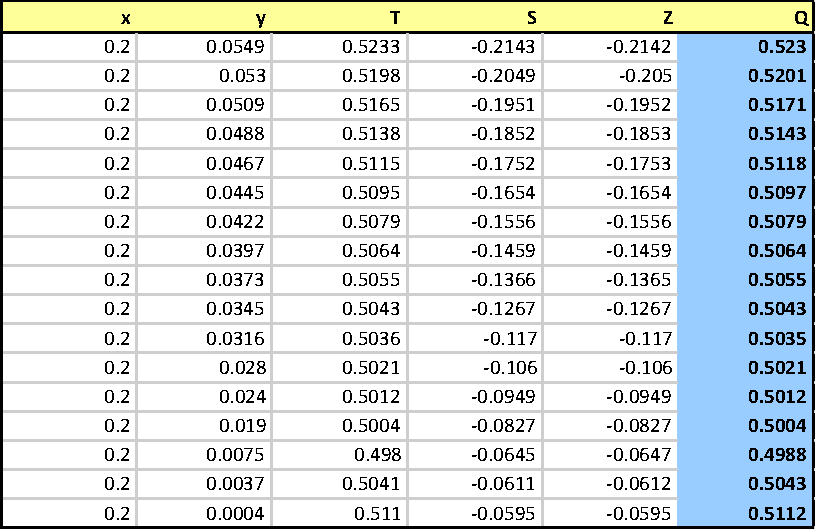
\includegraphics[width=13cm]{tableau}
\end{center}
\end{table}
%~~~~~~~~~~~~~~~~~~~~~~~~~~~~~~~~~~~~~~~~

\section{Conclusion}

Toute bonne chose a une fin.


\begin{thebibliography}{9}

\bibitem{bib:einstein}
F. Einstein, {\it I, Robot}, Journal of Medical Errors {\bf 126}, 132 (1818).

\bibitem{bib:rutherford}
E. Rutherford, {\it The Scattering of $\alpha$ and $\beta$ Particles by Matter and the Structure of the Atom}, Philosophical Magazine, \textbf{21}, 669 (1911)


\end{thebibliography}
%===============================================================================
\end{document}
